
\documentclass[conference]{IEEEtran}
\IEEEoverridecommandlockouts
\usepackage{cite}
\usepackage{amsmath,amssymb,amsfonts}
\usepackage{algorithm}
\usepackage{algpseudocode}
\usepackage{graphicx}
\usepackage{textcomp}
\usepackage{xcolor}
\usepackage{float}
\def\BibTeX{{\rm B\kern-.05em{\sc i\kern-.025em b}\kern-.08em
    T\kern-.1667em\lower.7ex\hbox{E}\kern-.125emX}}
\algnewcommand{\algorithmicand}{\textbf{ and }}
\algnewcommand{\algorithmicor}{\textbf{ or }}
\algnewcommand{\OR}{\algorithmicor}
\algnewcommand{\AND}{\algorithmicand}
\algnewcommand{\var}{\texttt}

\begin{document}
\title{8 Puzzle Problem}
\author{\IEEEauthorblockN{1\textsuperscript{st} Raunak Rathore}
\IEEEauthorblockA{\textit{Information Technology} \\
\textit{IIIT Allahabad}\\
Prayagaraj, India \\
iit2019222@iiita.ac.in}
\and
\IEEEauthorblockN{2\textsuperscript{nd} Prince Kumar Gupta}
\IEEEauthorblockA{\textit{Information Technology} \\
\textit{IIIT Allahabad}\\
Prayagaraj, India \\
iit2019223@iiita.ac.in}
\and
\IEEEauthorblockN{3\textsuperscript{rd} Shivangi Verma}
\IEEEauthorblockA{\textit{Information Technology} \\
\textit{IIIT Allahabad}\\
Prayagaraj, India \\
iit2019224@iiita.ac.in}
}
\maketitle

\begin{abstract}
This paper introduces an algorithm to Solve the 8 Puzzle Problem. The idea is to list down and analyze different approaches to find the most efficient solution in terms of time and space complexity.
\end{abstract}

\begin{IEEEkeywords}
Branch and Bound, Breadth First Search

\end{IEEEkeywords}

\section{Introduction}

The 8 Puzzle Problem states that given a 3×3 board with 8 tiles (every tile has one number from 1 to 8) and one empty space. The objective is to place the numbers on tiles to match the final configuration using the empty space. We can slide four adjacent (left, right, above, and below) tiles into the empty space. We will be making use of Branch and Bound algorithm to solve the problem.
\\
\\
\textbf{Branch and Bound: } The search for an answer node can often be speeded by using an “intelligent” ranking function, also called an approximate cost function to avoid searching in sub-trees that do not contain an answer node. It is similar to the backtracking technique but uses a BFS-like search.\\\\
\textbf{Breadth First Search: } BFS is a traversing algorithm where you should start traversing from a selected node (source or starting node) and traverse the graph layerwise thus exploring the neighbour nodes (nodes which are directly connected to source node). You must then move towards the next-level neighbour nodes.\\

As the name BFS suggests, you are required to traverse the graph breadthwise as follows:\\
1. First move horizontally and visit all the nodes of the current layer.\\
2. Move to the next layer.

\section{Algorithm Design}
While evaluating and traversing through the tree, we will come across three different types of nodes. These nodes are: Live Node, E-Node and Dead Node.\\\\
Following is a short description of these nodes:\\
\textbf{Live Node: } It is a node that has been generated but whose children have not yet been generated. \\\\
\textbf{E-Node: } It is a live node whose children are currently being explored. In other words, an E-node is a node currently being expanded.  \\\\
\textbf{Dead Node: } It is a generated node that is not to be expanded or explored any further. All children of a dead node have already been expanded. \\\\
% \begin{figure}[htbp]
%     \centering
%     \includegraphics[scale = 0.50]{Breaking Into Triangles.jpeg}
%     \caption{Breaking Into Triangles}
% \end{figure}
Next, how do we decide when to follow which particular node and when to avoid a different node? There has to be some way to know following which path will give the best result. This is done by calculating cost of each node. Cost of a node depicts how difficult will it be to reach the solution when following this particular path. Hence, lesser the cost, better the solution.\\\\
\textbf{Cost Function }\\Each node X in the search tree is associated with a cost. The cost function is useful for determining the next E-node. The next E-node is the one with the least cost.\\
\\

Now let us determine the cost function for our 8 puzzle problem. Let us assume that moving one tile in any direction will have a 1 unit cost. Keeping that in mind, we define a cost function for the 8-puzzle algorithm as below: \\

c(x) = f(x) + h(x) where\\\\
f(x) is the length of the path from root to x (the number of moves so far) and\\
h(x) is the number of non-blank tiles not in their goal position (the number of misplaced tiles). There are at least h(x) moves to transform state x to a goal state\\

Let us try to solve an example first and then frame the algorithm. Consider the initial (left) and final state (right) as shown below:\\
\begin{figure}[htbp]
    \centering
    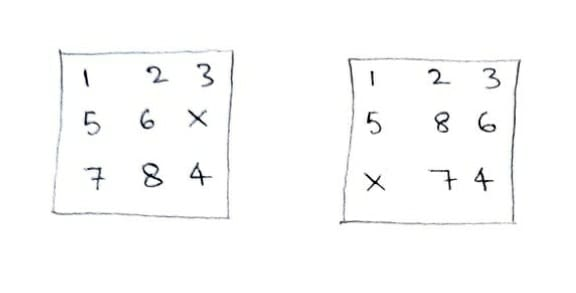
\includegraphics[scale = 0.45]{InitialvsFinal.jpeg}
    \caption{Initial vs Final State}
\end{figure}\\


Now, the empty tile (depicted by cross) can move in three directions: up, left and down. However to attain the final state, it is best if the tile shifts to its left. (See Fig. 2),Because in left move effective cost is 4 whereas in up and down it is 6.we will proceed to that which has least cost among all and leave the rest. \\
\begin{figure}[htbp]
    \centering
    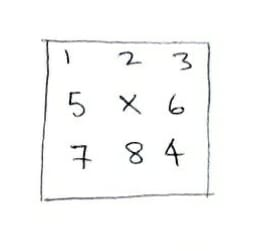
\includegraphics[scale = 0.50]{step1.jpeg}
    \caption{Step 1}
\end{figure}\\


Similarly, the empty tile (depicted by cross) can move in all four directions but not in the right direction because if we move empty tile in right direction we get the parent one so except right move we will move in all possible direction. However to attain the final state, it is best if the tile shifts downwards(same reason least effective cost).(See Fig. 3).\\
\begin{figure}[htbp]
    \centering
    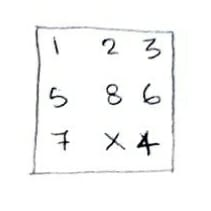
\includegraphics[scale = 0.50]{step2.jpeg}
    \caption{Step 2}
\end{figure}\\

Now,for the left move value of h(x) will be zero, means all non-blank tiles are in their goal position and that is how to attain the final state. (See Fig. 4).
\begin{figure}[htbp]
    \centering
    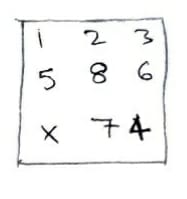
\includegraphics[scale = 0.50]{step3.jpeg}
    \caption{Step 3}
\end{figure}\\

Following is the psuedo-code implementing above algorithm:\\
\begin{algorithm}
\caption{LCSearch Function}
    \label{fup}
    \begin{algorithmic}[1]
    \Function{LCSearch}{$list_node *t$}
        \If {t is an answer node}
            \State print(t)
            \State \textbf{return} 
        \EndIf
        
        \State E = t; // E-node
        \State Initialize the list of live nodes to be empty;
        \State
        \State \textbf{while} $(true)$ 
        \State \textbf{for} each child $x$ of $E$ 
                
                \If{x is an answer node}
                    \State print(path from x to t)
                    \State \textbf{return}
                \EndIf
                \State Add (x); // Add x to list of live nodes;
                \State x$->$parent = E; // Pointer for path to root
        \State \textbf{end for}
        
        \State
        \If{there are no more live nodes}
            \State print("No answer node")
            \State \textbf{return}
        \EndIf
        \State
        \State// Find a live node with least estimated cost
        \State E = Least(); 

        \State // The found node is deleted from the list of 
        \State // live nodes
        
        \State \textbf{end while}
        
        
    \EndFunction
  \end{algorithmic}
\end{algorithm}

\section{Analysis}


\textbf{Time Complexity:} \\
Time complexity - 
 We keep running the BFS-like search until the destination state is not reached. For each state we generate an average of three new children and if the final state is found at a depth of D then the number of nodes generated will be (avg-number-of-children)D.

Avg no of children = (corner-points*2 + middle-point*4 + edge-middle-point*3)/9
		=   (4*2+1*4+4*3)/9  =  2.66 
Since the weightage of the middle point will be more, we can approximate it to 3. 

So, the worst time complexity will be O(3D) where D is the depth of the final state from initial state.

The best case time complexity will be O(1) when either the solution is not possible or the initial state is equal to the final state. 

\textbf{Space Complexity:} \\

Space complexity will be equal to the number of nodes traversed*size-of-one-state. 

So, Worst case space complexity = O(9!*size-of-one-state). 

Best case space complexity will be O(1) when either the initial state and final states are the same or the solution is not feasible.

\\
\section{Conclusion}
We implemented the given problem in the optimized way under certain constraints.

\end{document}
